\section{Tecnologie}

\subsection{Introduzione}

\begin{frame}{Tecnologie utilizzate}

\begin{itemize}
\item JBoss AS 7.1
	\begin{itemize}
	\item fornisce l'infrastruttura per consentire l'esecuzione di una web application
	\end{itemize}

\item Java EE 6
	\begin{itemize}
	\item piattaforma software per lo sviluppo di applicazioni enterprise
	\item comprende varie tecnologie, fra cui:
		\begin{itemize}
		\item JPA (Java Persistence API) 2.0
		\item CDI (Contexts and Dependency Injection) 1.0
		\item JSF (JavaServer Faces) 2.0
		\end{itemize}
		
	\end{itemize}

\end{itemize}


\end{frame}

\begin{frame}{Bean}

\begin{itemize}
\item Sono componenti software riusabili che possono essere gestiti dal container

\item Vari tipi:
	\begin{itemize}
	
	\item \textsl{Enterprise JavaBeans} (EJB): bean utilizzati per la logica di business o la persistenza
		\begin{itemize}
		\item session bean
		\item message-driven bean
		\item entity bean
		\end{itemize}
		
	\item  \textsl{Managed beans}: bean utilizzati a livello di presentazione
	\end{itemize}

\end{itemize}

\end{frame}


\subsection{JPA}
\begin{frame}{Java Persistence API}

\begin{itemize}
\item Si occupa della persistenza dei dati
\end{itemize}

\begin{itemize}
\item Problema:

	\begin{itemize}
	\item Nelle applicazioni enterprise è necessario ricorrere ad un database
	
	\item Il modello più utilizzato all'interno dei database è il \textsl{modello relazionale}
		\begin{itemize}
		\item le entità sono le \textsl{relazioni}
		\item sono collegate tra di loro mediante \textsl{chiavi}
		\end{itemize}
	
	\item Il modello utilizzato all'interno delle applicazioni Java è il \textsl{modello a oggetti}
		\begin{itemize}
		\item le entità sono le \textsl{classi}
		\item sono collegate tra di loro mediante \textsl{riferimenti}
		\end{itemize}
	
	\end{itemize}

\end{itemize}

\end{frame}


\begin{frame}{Integrazione fra i modelli}

\begin{itemize}
\item Occorre un sistema per la conversione tra i due modelli

	\begin{itemize}
	\item non deve influire pesantemente sullo sviluppo dell'applicazione
	\item in particolare, deve garantire:
	
		\begin{itemize}
		\item trasparenza rispetto al modello di dominio
		\item recupero di informazioni indipendente dal database
		\item compatibilità con database preesistenti
		\end{itemize}
	
	\end{itemize}

\end{itemize}

\end{frame}


\begin{frame}{Costrutti fondamentali}

\begin{itemize}
\item Entità
	\begin{itemize}
	\item è un'unità che possiede uno stato e può essere persistita
	\item una classe Java è un'entità se:
		\begin{itemize}
		\item è annotata \texttt{@Entity}
		\item ha un costruttore senza parametri
		\end{itemize}
	\end{itemize}

\item Entity Manager
	\begin{itemize}
	\item gestisce le entità
	\item è associato ad un \textsl{Persistence Context}
		\begin{itemize}
		\item è l'insieme delle entità gestite da un Entity Manager in un dato momento
		\item se un entità fa parte di un Persistence Context viene detta \textsl{managed}
		\item altrimenti viene detta \textsl{detached}
		\end{itemize}
	\end{itemize}

\end{itemize}	


\end{frame}

\begin{frame}{Query}

\begin{itemize}
\item Si usa il \textsl{Java Persistence Query Language} (JPQL)

\item Sintassi simile a SQL, ma:

	\begin{itemize}
	\item è indipendente dal database
	\item utilizza le entità del modello di dominio e relativi attributi
	\end{itemize}


\end{itemize}

\end{frame}


\subsection{CDI}

\begin{frame}{Contexts and Dependency Injection}

\begin{itemize}
\item Problema: incompatibilità tra
	\begin{itemize}
	\item il livello di business, che usa EJB;
	\item il livello di presentazione, che usa Managed bean.
	\end{itemize}
	
\item CDI:
	\begin{itemize}
	\item consente l'utilizzo di EJB nel livello di presentazione
	\item fornisce una specifica per la definizione di Managed bean
	\end{itemize}
\end{itemize}

\end{frame}



\begin{frame}{Panoramica}

\begin{itemize}
\item Servizi offerti:
	\begin{itemize}
	\item Contesto
	\item Iniezione di dipendenza
	\end{itemize}

\item Caratteristiche principali:
	\begin{itemize}
	\item integrazione Expression Language
	\item disaccoppiamento
	\item controllo sui tipi
	\end{itemize}
\end{itemize}

\end{frame}

\begin{frame}{Bean CDI}

\begin{itemize}
\item \textsl{Scope}
	\begin{itemize}
	\item lega il bean ad un particolare contesto
	\item determina il ciclo di vita
	\item limita la visibilità al client
	\end{itemize}
	
\item 4 possibili scope:
	\begin{itemize}
	\item Request
	\item Conversation
	\item Session
	\item Application
	\end{itemize}

\end{itemize}

\end{frame}



\subsection{JSF}

\begin{frame}{JavaServer Faces}

\begin{itemize}
\item Framework per lo sviluppo di interfaccia grafica
\item \textsl{Component-based}
\item Consente estensione delle funzionalità tramite librerie di terze parti
\end{itemize}

\end{frame}


\begin{frame}{Architettura}

\begin{itemize}
\item Architettura Model-View-Controller
\end{itemize}

\begin{figure}
	\centering
	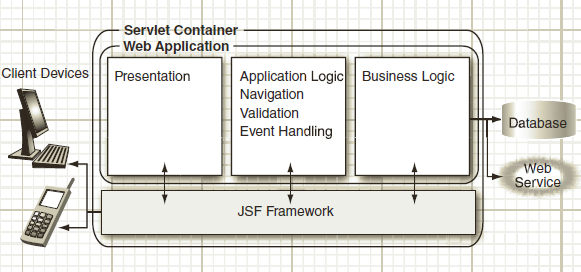
\includegraphics[width=0.5\textwidth]{JSF_architecture.png}
\end{figure}

\end{frame}


\begin{frame}{Comunicazione client-server}
\begin{figure}
	\centering
	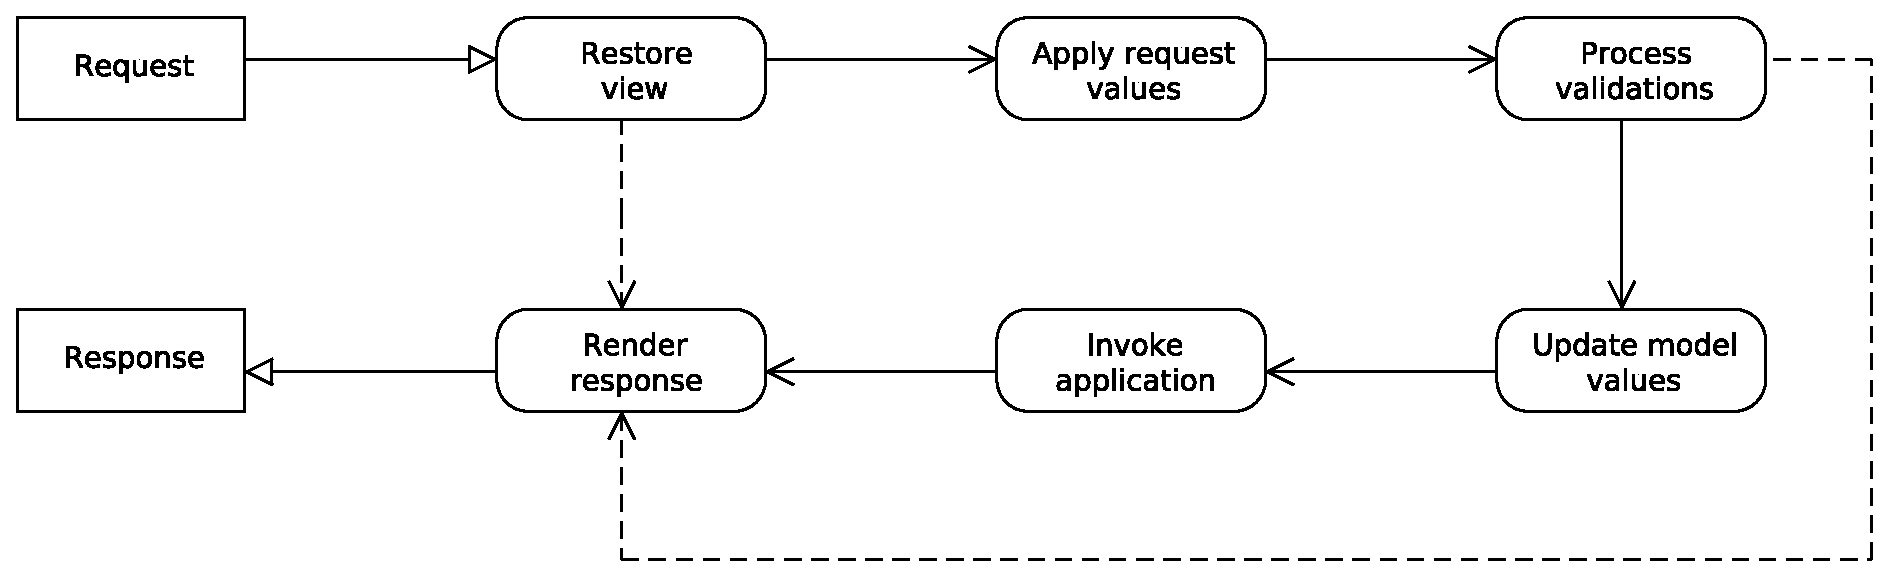
\includegraphics[width=1\textwidth]{custom_JSF_lifecycle.eps}
\end{figure}

\end{frame}
























